% -*- mode: latex; mode: flyspell; ispell-local-dictionary: "en_US"; coding: utf-8; fill-column: 80 -*-

\documentclass{article}

\usepackage[utf8]{inputenc}
\usepackage[english]{babel}

\usepackage{amsmath,amsfonts,amssymb}
\usepackage{fullpage}
\usepackage{verbatim}

\usepackage{tikz,pgfplots}

\pgfplotsset{
  width=150mm,height=100mm,
  major grid style={thin,dotted,color=black!50},
  minor grid style={thin,dotted,color=black!50},
  grid,
  every axis/.append style={
    line width=0.5pt,
    tick style={
      line cap=round,
      thin,
      major tick length=4pt,
      minor tick length=2pt,
    },
  },
  legend cell align=left,
  legend pos=north west,
}

%%%%%%%%%%%%%%%%%%%%%%%%%%%%%%%%%%%%%%%%%%%%%%%%%%%%%%%%%%%%%%%%%%%%%%%%%%%%%%%%

\begin{document}

\title{Sorting Speed Example}
\author{Timo Bingmann}
\maketitle

% IMPORT-DATA stats stats.txt

\begin{center}
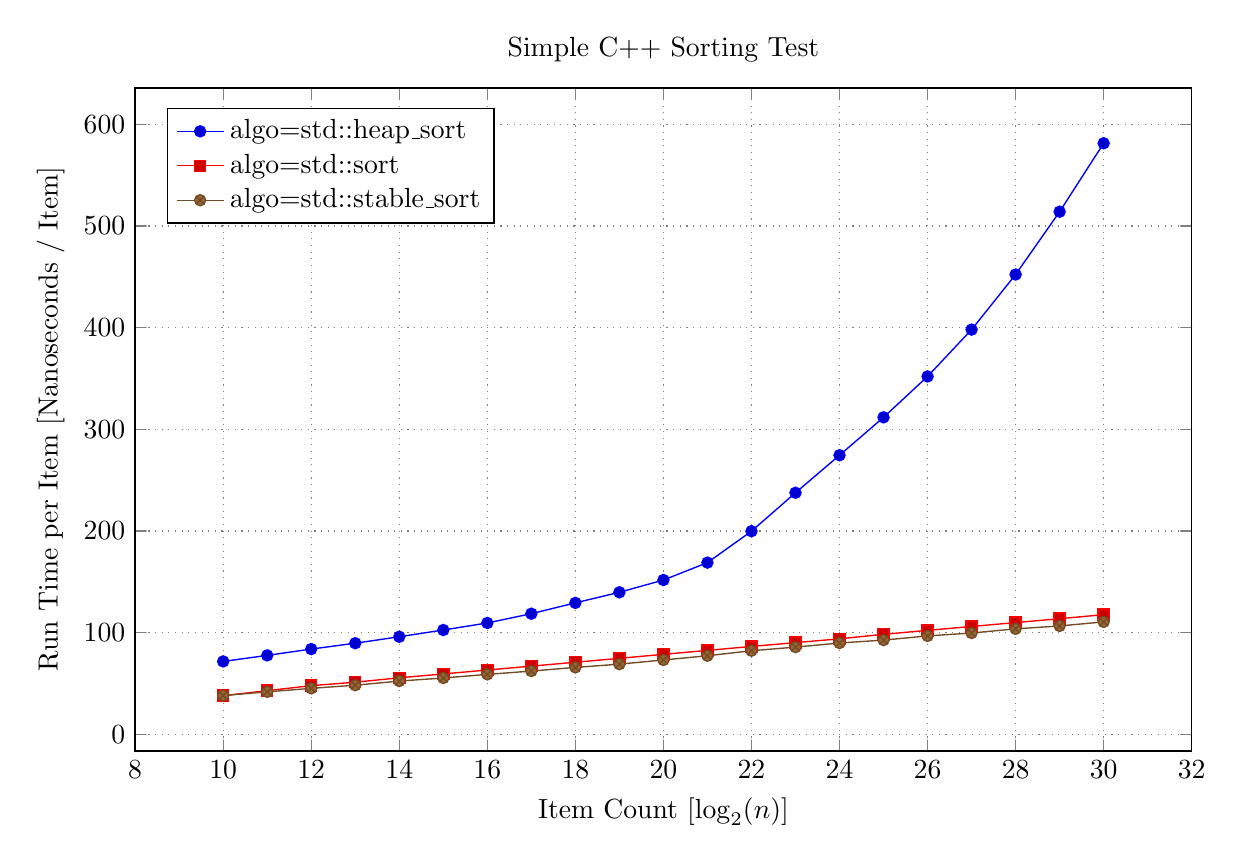
\begin{tikzpicture}
  \begin{axis}[
    title={Simple C++ Sorting Test},
    xlabel={Item Count [$\log_2(n)$]},
    ylabel={Run Time per Item [Nanoseconds / Item]},
    ]

    %% MULTIPLOT(algo) SELECT LOG(2, size) AS x, MEDIAN(time / repeats / size * 1e9) AS y, MULTIPLOT
    %% FROM stats GROUP BY MULTIPLOT,x ORDER BY MULTIPLOT,x
    \addplot coordinates { (10,71.6615) (11,77.5939) (12,83.8065) (13,89.5691) (14,95.9241) (15,102.562) (16,109.495) (17,118.608) (18,129.266) (19,139.672) (20,151.737) (21,168.85) (22,199.766) (23,237.565) (24,274.479) (25,311.786) (26,352.004) (27,398.075) (28,452.284) (29,514.045) (30,581.396) };
    \addlegendentry{algo=std::heap\_sort};
    \addplot coordinates { (10,37.9929) (11,42.9001) (12,47.8324) (13,51.2096) (14,55.5614) (15,59.3466) (16,63.2313) (17,67.0138) (18,70.8553) (19,74.6909) (20,78.6448) (21,82.4893) (22,86.4092) (23,90.1377) (24,93.8964) (25,98.3199) (26,102.219) (27,106.035) (28,109.866) (29,113.705) (30,117.649) };
    \addlegendentry{algo=std::sort};
    \addplot coordinates { (10,38.0611) (11,41.7566) (12,45.1556) (13,48.2661) (14,52.3302) (15,55.3477) (16,58.915) (17,62.1703) (18,65.7791) (19,68.9638) (20,73.0819) (21,77.2482) (22,82.1805) (23,85.7273) (24,89.7738) (25,92.6328) (26,96.7431) (27,99.6031) (28,103.699) (29,106.563) (30,110.559) };
    \addlegendentry{algo=std::stable\_sort};

  \end{axis}
\end{tikzpicture}
\end{center}

\begin{table}\centering
\begin{tabular}{l|rrr}
$n$ & \texttt{std::sort} & \texttt{std::stable\_sort} & STL heap sort \\ \hline
%% TABULAR REFORMAT(col 1-3=(precision=1) row 0-100=(min=bold))
%% SELECT '$2^{' || FLOOR(LOG(2, size)) || '}$' AS x,
%% (SELECT MEDIAN(time / repeats / size * 1e9) FROM stats s1 WHERE s1.algo='std::sort' AND s1.size = s.size GROUP BY s1.size),
%% (SELECT MEDIAN(time / repeats / size * 1e9) FROM stats s1 WHERE s1.algo='std::stable_sort' AND s1.size = s.size GROUP BY s1.size),
%% (SELECT MEDIAN(time / repeats / size * 1e9) FROM stats s1 WHERE s1.algo='std::heap_sort' AND s1.size = s.size GROUP BY s1.size)
%% FROM stats s
%% GROUP BY s.size ORDER BY s.size
$2^{10}$ & \bf 38.0 &      38.1 &  71.7 \\
$2^{11}$ &     42.9 &  \bf 41.8 &  77.6 \\
$2^{12}$ &     47.8 &  \bf 45.2 &  83.8 \\
$2^{13}$ &     51.2 &  \bf 48.3 &  89.6 \\
$2^{14}$ &     55.6 &  \bf 52.3 &  95.9 \\
$2^{15}$ &     59.3 &  \bf 55.3 & 102.6 \\
$2^{16}$ &     63.2 &  \bf 58.9 & 109.5 \\
$2^{17}$ &     67.0 &  \bf 62.2 & 118.6 \\
$2^{18}$ &     70.9 &  \bf 65.8 & 129.3 \\
$2^{19}$ &     74.7 &  \bf 69.0 & 139.7 \\
$2^{20}$ &     78.6 &  \bf 73.1 & 151.7 \\
$2^{21}$ &     82.5 &  \bf 77.2 & 168.9 \\
$2^{22}$ &     86.4 &  \bf 82.2 & 199.8 \\
$2^{23}$ &     90.1 &  \bf 85.7 & 237.6 \\
$2^{24}$ &     93.9 &  \bf 89.8 & 274.5 \\
$2^{25}$ &     98.3 &  \bf 92.6 & 311.8 \\
$2^{26}$ &    102.2 &  \bf 96.7 & 352.0 \\
$2^{27}$ &    106.0 &  \bf 99.6 & 398.1 \\
$2^{28}$ &    109.9 & \bf 103.7 & 452.3 \\
$2^{29}$ &    113.7 & \bf 106.6 & 514.0 \\
$2^{30}$ &    117.6 & \bf 110.6 & 581.4 \\
% END TABULAR SELECT '$2^{' || FLOOR(LOG(2, size)) || '}$' AS x, (SELECT MEDI...
\end{tabular}
\caption{Runtime per element for different sorting implementation, median of 15 runs.}
\end{table}

\begin{comment}
% TEXTTABLE SELECT COUNT(*), SUM(time) FROM stats
+-------+-------------+
| count |         sum |
+-------+-------------+
|   945 | 25661.41392 |
+-------+-------------+
% END TEXTTABLE SELECT COUNT(*), SUM(time) FROM stats
\end{comment}

\end{document}

%%%%%%%%%%%%%%%%%%%%%%%%%%%%%%%%%%%%%%%%%%%%%%%%%%%%%%%%%%%%%%%%%%%%%%%%%%%%%%%%
